\documentclass[../report.tex]{subfiles}

\begin{document}

\subsection{Requirements}
As stated in the introduction, the aim of the application was to be able to render a virtual scene in 3D using `photo-realistic techniques', 
as the term `realism' carries some degree of subjectivity, we decided it was best to implement some of the most commonly believed aspects of PBR and leave the rating of
rendering realism as an exercise to the viewer. \\

The application was designed to run on all modern desktop platforms, specifically Windows, Linux and MacOS.\ To facilitate this, any code that
would be platform specific is instead handled by third-party libraries,
however, due to the nature of the chosen programming 
language, Rust, the final output is produced as a native executable, therefore, 
multiple versions of the application would have to be compiled for each platform
that the application should run on, there are multiple ways to do this, including compiling the code on a native machine or inside a virtual machine, 
however the Rust compiler system provides a fairly simple system for cross-compilation, which will allow me to set up the project once and compile for multiple platforms. \\


The actual performance of the rendering algorithms themselves were of a secondary concern, although the use of lower level programming languages and APIs allow 
for more capability for optimisation techniques than a higher level of abstraction that one may find in a modern game engine like Unity or Unreal Engine, for instance. 
Performance in this case specifically refers to the amount of time it takes to render a frame and display it to the screen, 
generally referred to as `frame time', it is the reciprocal of the more commonly used term `FPS' (frames per second), 
if a scene can be rendered in at 24 frames per second (approx. 0.417 seconds per frame) it is considered to be rendering in real-time \mycite{unity-real-time} \\

we decided that performance shouldn't be the main focus because any measure of performance would be somewhat hardware dependant, as a less optimised system 
could run better on more powerful hardware, and vice-versa, therefore it would be difficult to get an objective view of the 
performance of the application without extensive testing on different systems; moreover the ability to perform ray-tracing 
in real-time has only recently been made available on consumer grade hardware at the time of writing, and the amount of extra
implementation required could potentially double or triple the potential workload, as this article attempts to show \mycite{year-of-real-time-ray-tracing}.

The final product was designed purely to be a showpiece and a proof of concept that the user will have very little interaction with, beyond just observing the output, despite this, there are 
still some safety concerns to be aware of; there are certain visual patterns that, when viewed, can trigger certain ailments or conditions, ranging from light headaches to epileptic seizures.
To minimise the risk of harmful effects, Microsoft outlines these patterns which should be avoided at all costs \mycite{xbox-epilepsy}.

\begin{itemize}
    \item{\emph{Luminance Flash}: A 10\% change in luminance (where 100\% luminance is a white screen). }
    \item{\emph{Red flash}: Similar to a luminance flash, but can occur with lower changes in luminance (when the change in value of (red - blue - green) * 320 is greater than 20)}
    \item{\emph{Spatial Pattern failure}: alternating bands with high contrast (more than 10\% contrast)}
\end{itemize}



\subsection{System Design}
we decided to use Rust as the implementation language because it is a relatively lower level language (compared to languages like Javascript and Python)
which would allow me to have tighter control of the underlying hardware while still maintaining a level of memory safety without having to sacrifice runtime performance with things like garbage collection, thanks to Rust\'s static memory guarantees, and C FFI compatibility allowed me to use all of the libraries that we wanted to use, moreover we could compile my final result into a single executable with statically linked dependencies. \\

Likewise, we decided to use Vulkan as the graphics API because Vulkan places strong emphasis on being explicit with its code, and requires that every part of the graphics pipeline be defined and configured beforehand, which gave strong insights into the work the graphics API does with the hardware behind the scenes, however the downside of this is that Vulkan becomes much more difficult to learn and use, compared to other options such as OpenGL.
The gulf in complexity is shown best through the `time to triangle' which is the time it takes to write code that allows the hardware to start displaying graphics, where OpenGL has a time to triangle of approximately 30 minutes, whereas Vulkan has a time to triangle of around a week \mycite{time-to-triangle}.

\begin{figure}[h]
    \centering
    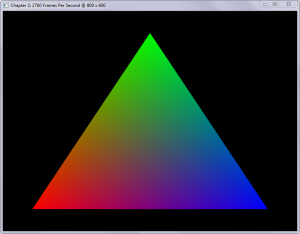
\includegraphics[width=0.5\textwidth]{images/triangle.png}
    \caption{An example of the triangle}
\end{figure}

Vulkan's core API is written in C, which means we had to choose bindings to allow my code to use the API, and we had a few options in this regard, ranging from machine generated bindings, to complete re-imaginings of the interface, ultimately, after much testing and experimentation, we decided to use Ash as my bindings library, because it struck a good middle ground between two extremes, it had code to make the language fit better into Rust, so we didn't have to spend too much time having to adapt the C API to fit better into the language, but it was still similar enough to the original API that we could still use the official documentation for help writing code.

We chose the SDL2 library for handling windowing, because it is a simple but mature library that is compatible with Vulkan out of the box, and because all we needed to do was create a window and retrieve some information from it, setup was fairly simple in this regard, using this library allowed me to write platform independent windowing code, without having to call OS specific functions in my code explicitly.

Linear algebra is an essential mathematical requirement for 3D rendering, particularly matrices and matrix transformations, and are used mainly for projecting the 3D image into 2D, and for handling transformations in 3D space. Because linear algebra is very complicated and potentially very easy to get wrong, and because the specific implementation details aren't very relevant to the core aim of the project, we used a library to provide this, called Nalgebra, as the most complete and fully featured linear algebra library for Rust, as well as an optional dependency that provides a more glm-like interface, which is the library of choice for graphics implementations in C/C++, and would help greatly when looking at external resources, that are most likely using C++ with glm.

We elected to use an iterative design process when designing and implementing the application, similar to the Spiral model, wherein we would plan a small section or aim to achieve a goal, and then build on that substrate. For example for one iteration, we would aim to render a simple graphic onto the screen, by writing the minimum amount of code that is needed to achieve that goal, then for the next iteration, we would focus on refactoring and re-writing the code we wrote earlier, in order to make the codebase easier to expand and add onto for later iterations.
This method allows me to plan and write code in manageable chunks, that can be individually implemented and then tested, as opposed to writing code in large chunks, that we would then have to spend large amounts of time debugging and tweaking parameters, without knowing where exactly the bug or bugs could be.

\subsection{Implementation}

\subsubsection{Project Setup}
The first thing we did was setting up the project. we uses `Cargo' (Rust's inbuilt package manager), to generate a basic project outline, running the command `cargo new project' generated a folder called project, which contained a `Cargo.toml' file and a `src' folder, containing the `main.rs' file.
The toml file is a text file that dictates the parameters of the project, such as the name of the executable, and which libraries that need to be downloaded from the core repository, and linked with the project.
The `main.rs' file is a Rust source file, and contains 
\mint{rust}|fn main() {}|
which is the entry point for the application, or put more simply, where the code starts.

\subsubsection{Window creation}
Once the project is set up, we worked on getting the window to show, and stay on the screen. The SDL library made this a fairly simple process, we created a new SDL context, and initialised the video subsystem, at that point, we could then create the window itself.

\begin{figure}[h]
    \centering
    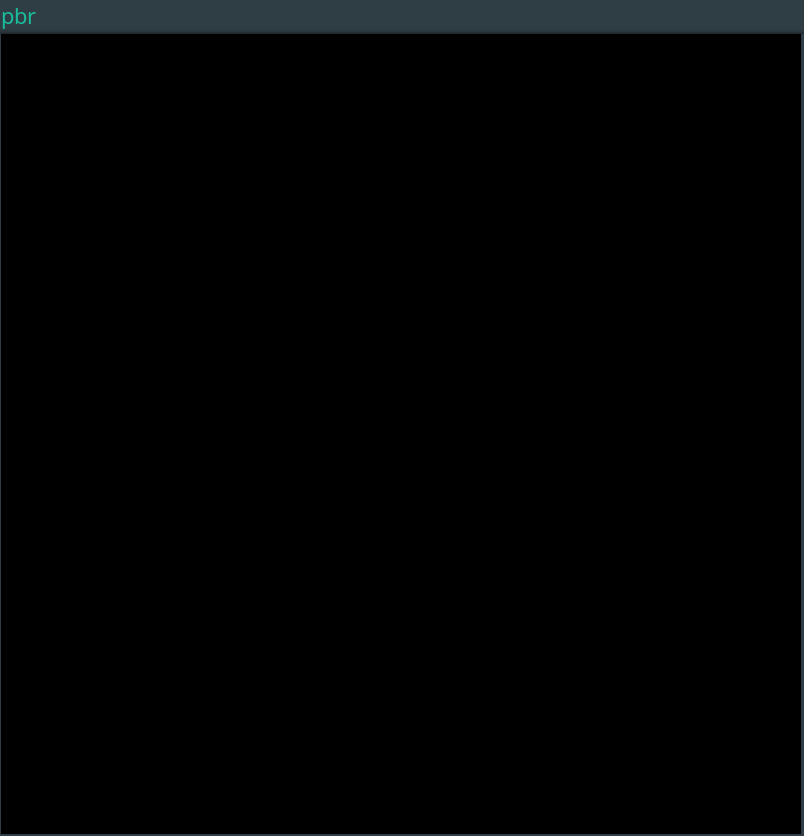
\includegraphics[width=0.25\textwidth]{images/blank_window.png}
    \caption{A window is created}
\end{figure}

At this point, we could construct a new Window object, specifying the width, height and window title.
During window creation we made sure to request Vulkan compatibility, which we would then retrieve at a later date.

At this point the window would show for a split second, before the program closed, this was because the main function had finished, which causes the program to end and clean itself up, to keep the window open we had to create a loop that runs until the window is closed, at which point the program can begin cleaning itself up, a basic example would be something like this:

\begin{minted}{rust}
fn main() {
    let window = Window::new();
    while window.open() {
        //do window things
    }
}
\end{minted}

However, at this point there are two issues, firstly, the program does not wait in between loops, so it will run as fast as it possibly can, and much faster than we need, secondly, we want to be able to control the window and respond to events such as keyboard and mouse input, to do this we needed to create an event loop, that polls the window each loop, to see if any events have been pushed to the queue, then handle it in our loop. At this moment, we need to handle the `Quit' event, we check if the received event is a Quit event, and if so, we close the loop, ending the program. 
As for the loop timing, we could set a limit at this point by timing how long it takes to do one loop, and then sleep (freeze the loop) so that each loop takes at least 16.6 milliseconds, or 60 loops per second, but we decided it would be better to let the hardware handle timing instead.

\subsubsection{Vulkan setup}
Once the window is up and the window loop is established, we could start setting up Vulkan, as mentioned in previous chapters, Vulkan is very explicit with its setup, so there was a fairly significant amount of setup that needs to be done before anything could be rendered, at this point in time, it would take approximately 1000 lines of code just to render a basic triangle.

The first thing that needed to be done in Vulkan was loading the functions that we were going to use, as is common in graphics APIs, this is because these APIs will often come with extra features or extensions that are specific to certain kinds of hardware, and the API gives you the option of loading these extensions and using them in a project, however most of these are non-standard and there is no guarantee that they will exist on every system you want to run the application on, we have no plans to pull in any hardware specific extensions beyond the standard ones that are required.

At this point we also request version 1.0.0 of the Vulkan API, although it is not the newest version of the API, it is much more likely to be available on most current consumer hardware, whereas requesting newer versions will limit which systems this code can run on, which would be an unnecessary restriction as we don't require any features from the newer versions.

Once the API was initialised, we could start loading the required extensions for the application, as polling for currently existing extensions on the host system is an OS level function, we relied on SDL to provide those for us, once we had a list of all available extensions on the system, we looped through each one to look for the specific extension we required, specifically the `swapchain' extension.
Although Vulkan is used mainly as a graphics API, that isn't its only function, Vulkan has compute capability, meaning it can use the GPU to process large amounts of mathematical data, therefore Vulkan has to have the ability to run on systems that aren't connected to a screen or able to render images, because of this, the ability to present images to the screen has to be loaded as an extension.

At this point, we also added the optional ability to enable a very handy feature of Vulkan called validation layers, these validation layers exist as a series of checks baked into the API calls, and when enabled, they will print messages to the terminal listing any warnings or errors that may have been inadvertently added into the software, however they do have a fairly strong impact on the runtime performance of the application, so we decided it was best to have it as a feature that could be turned on and off when needed.

It was at this point we enabled the `FIFO' presentation mode, which is often known colloquially as VSync, which made sure that the application never ran faster than the time it takes to refresh the screen.

\subsubsection{Device Selection}
Once the core API was setup and the functions were loaded, we started interfacing with the hardware, firstly we had to choose a physical device, which corresponds to the physical hardware capable of rendering graphics, although most people will only have one GPU in their system, some people will have multiple, so we needed to grade all of the available physical devices on how suitable they were for our purposes and choose that one.

We chose a very simple algorithm for determining the best device to use
\begin{minted}{rust}
fn choose_physical_device(instance: &Instance) -> vk::PhysicalDevice
{
    let physical_devices = unsafe{ 
        instance.enumerate_physical_devices()
    }.unwrap();

    let physical_device = *physical_devices.iter().max_by_key(|pd| {
        let mut score = 0u64;
        let props = unsafe{ instance.get_physical_device_properties(**pd) };

        //prioritize discrete gpus
        score += match props.device_type {
            PhysicalDeviceType::DISCRETE_GPU => 1000,
            PhysicalDeviceType::INTEGRATED_GPU => 100,
            PhysicalDeviceType::VIRTUAL_GPU => 10,
            PhysicalDeviceType::CPU => 5,
            _ => 1,
        };

        //prioritize highest vram
        score += props.limits.max_memory_allocation_count as u64;

        score
    }).unwrap();

    physical_device
}
\end{minted}
as shown above, we looped through each physical device on the system, and attributed a score to each, we prioritised selecting a discrete GPU over any integrated or virtualised GPU as they tend to be a lot lest powerful, also we prioritised the one with the highest amount of memory, as that tends to be correlated with performance.

\subsubsection{The swapchain}
Once we selected a suitable physical device, we started to look for device queues, the way Vulkan facilitates communication between the CPU and the GPU is through the use of programmable command buffers, commands are sent to the GPU asynchronously, and are placed in a queue, waiting for the GPU to execute them, Vulkan has multiple different types of queue, but we were interested in only two of them, the graphics queue, and the present queue, the graphics queue is responsible for handling all graphical data and operations, and the present queue is responsible for displaying images onto the screen. We enumerated through all of the queues and tested their features, saving the indices of the two queues that we were looking for.

Then we were able to construct the logical device, which is an abstraction over the physical hardware that Vulkan uses to handle most operations, from allocating memory to submitting commands.

After this, we queried the window surface for what formats it was able to render, as well as the size of the drawable surface,
with this information, we were then able to construct the swapchain.
The swapchain is a series of images, modern swapchains will have at least 2 images, but some can have more, in a 2 image swapchain (also called a double-buffered swapchain), one image is the primary buffer and contains the image currently being displayed on the screen, whereas the other image is the secondary buffer, and is the one that gets images written onto it, once the system has finished writing the image to the secondary buffer, it swaps the buffers around, so the secondary buffer becomes the primary and vice-versa. Older systems didn't use to have double buffering, and as a result you could often see the new image being rendered onto the screen line by line.

Then we defined the render pass, a render pass is when the GPU takes certain inputs and uses it to create an image, modern renderers often do multiple render passes per frame, for example, it may do one pass for colour, then a second pass for shadows, then a third for depth, after which the GPU will combine all of these passes (also known as compositing) into a single image for presenting, however at this stage we are just doing a single colour pass.

\subsubsection{Shader loading}
Shaders are source code designed to run on the GPU as part of the graphics pipeline, shaders are often written like code, particularly in a C-like shader language called GLSL (GL Shader Language), however, Vulkan expects its shader code in a compiled binary format called SPIR-V, to facilitate this, we decided to use a feature of Rusts called macros, specifically the `include-glsl' macro, that could import a glsl shader file, and convert it into SPIR-V as part of the build step, however Vulkan cannot use SPIR-V on its own, so we had to construct shader modules, that stored the shader data, but also told Vulkan how the shaders were supposed to be used.
Vulkan is able to support a wide variety of shaders, but we were only interested in two types of shader, the vertex shader and the fragment shader.
The vertex shader is responsible for letting the GPU know where points should exist in 3D space, whereas the fragment shader is responsible for dictating the appearance of the objects that are rendered, although at this stage, it is just setting the colours of each vertex.

\subsubsection{Creating the pipeline}
Putting together all of the previous information, we then constructed the graphics pipeline, the pipeline refers to the various processes by which the inputs get converted into an output, as a testament to its importance, the pipeline required a lot of setup, such as the vertex and fragment shader modules, information about the size of the renderable area (referred to as the viewport), colour blending information and how groups of vertices get filled to create faces.
Creating the pipeline is a very expensive process and should be minimised wherever possible.

\subsubsection{Command buffering}
After all the prior setup, we could then start sending commands to the GPU, 
firstly we allocated a buffer for each image in the swapchain, then we used these buffers to apply our shader input into the pipeline (as well as specifying which colour to clear the screen).
At this point we were almost able to render a triangle, but we first had to set up the synchronisation primitives, Vulkan has two main types of synchronisation primitive, the fence and the semaphore, the fence will block a thread, if its data is currently in use, whereas a semaphore will allow multiple sources to access its data at a single time, but will block if that number goes above a certain amount.

We used semaphores to alert us when an image was finished being rendered to, and when an image was made available to receive new input, we used the fences to prevent images from being written to by multiple concurrent sources, when an image was being written to it was referred to as `in flight'.

with the command buffers set up and properly synced, we could finally render our triangle.


\begin{figure}[h]
    \centering
    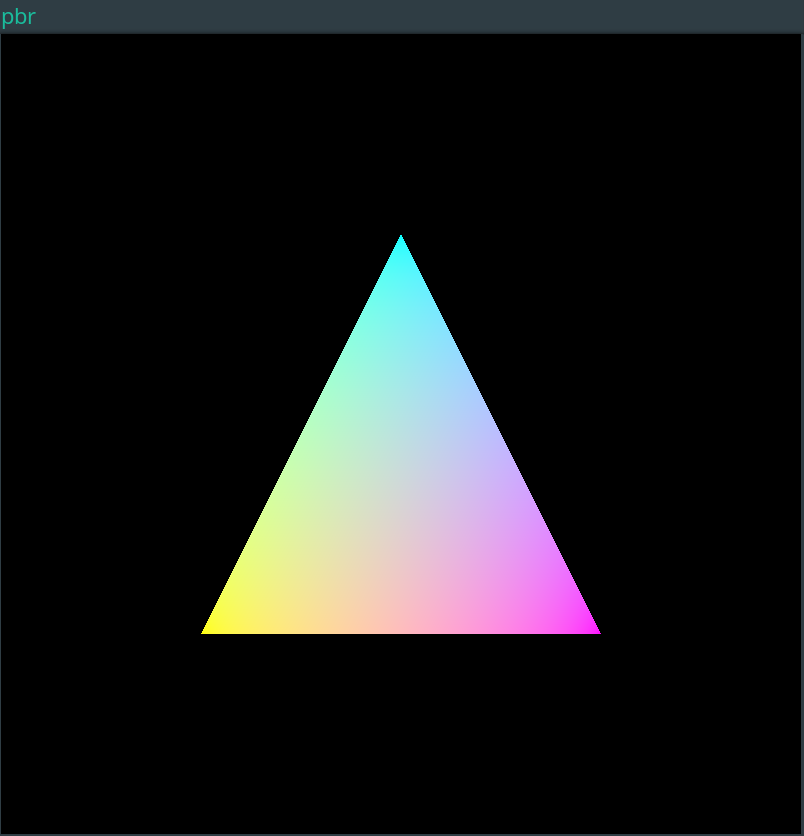
\includegraphics[width=0.25\textwidth]{images/window_triangle.png}
    \caption{A triangle is rendered, using secondary colours as vertex colours}
\end{figure}


\subsubsection{Index buffers}

At this point, we rendered a triangle onto the screen, and we were doing so by specifying three vertices, that the renderer would then link together and form a shape with a face, however if we wanted to render more complex shapes, we would have to either input vertices as groups of three, and end up sending large amounts of duplicate information to the GPU, or we could create an index buffer, which would be a collection of indices that each refer to a certain vertex, which is much more efficient.

\begin{figure}[h]
    \centering
    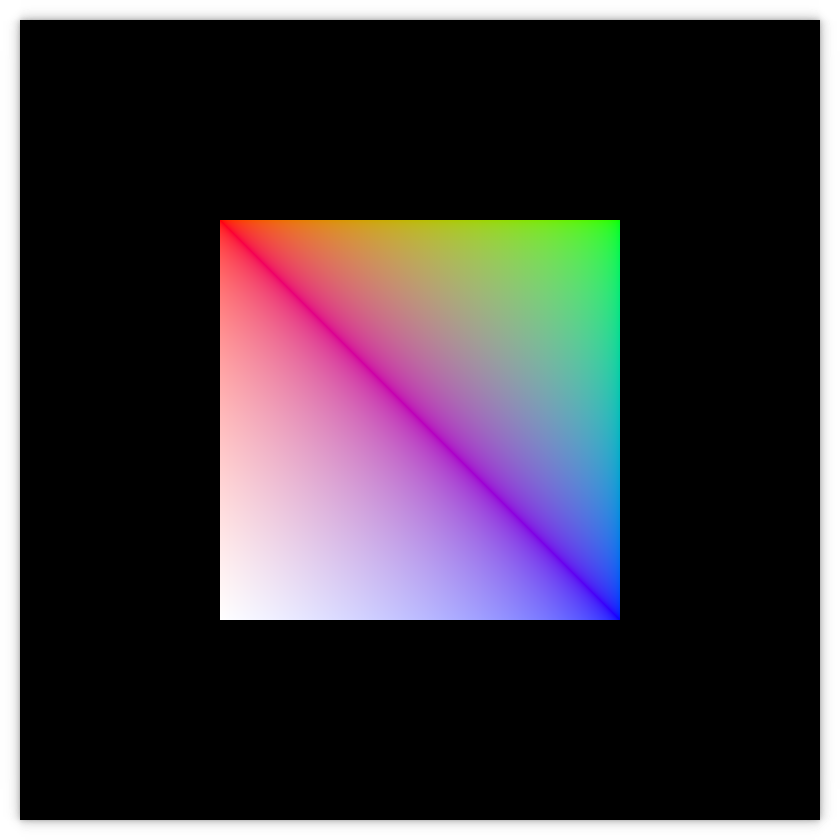
\includegraphics[width=0.25\textwidth]{images/index_buffers.png}
    \caption{A rectangle rendered using four vertices, linked with an index buffer}
\end{figure}

Even though the above image is rendered with triangles, we only provided four vertices to the GPU, had we used the old method, we would have had to provided six vertices, two of which would be repeated.

\subsubsection{Model-View-Projection}
In order to take our renderer from two-dimensional to three-dimensional, we had to introduce three four by four matrices, the model, the view and the projection matrices.
By performing a series of matrix transformations, you can take a flat 2D image and create the illusion of depth.

The model matrix is designed to `translate model space into world space' \mycite{mvp} and can transform an object and place it in the world, the model matrix is made up of an objects translation, rotation and scale vectors.

The view matrix positions an object relative to the camera, by manipulating the view matrix, you can give the appearance of a camera rotating around a fixed point, the view matrix also defines the up axis, which is often (but not always) positive Z.

The Projection matrix is used to give a scene a sense of perspective, with objects that are farther away appearing squished and following a vanishing point, without the projection matrix, the scene would appear flat.

The following shader code is an example of how MVP would be applied using a vertex shader.

\begin{minted}{glsl}
#version 450
#extension GL_ARB_separate_shader_objects : enable

layout(binding = 0) uniform UniformBufferObject {
    mat4 model;
    mat4 view;
    mat4 proj;
 } ubo;

layout(location = 0) in vec3 inPosition;



void main() {
    gl_Position = ubo.proj * ubo.view * ubo.model * vec4(inPosition, 1.0);
}
\end{minted}

\subsubsection{Staging buffers}
Before this point, we were creating buffers on the CPU and asking the GPU to read from them, and while this works, it is much slower than letting the GPU read its own data, to this end, we implemented staging buffers, whereby we would store our data in the buffer, just like before, however our new buffers would be marked with the `device local' flag, meaning the data would reside on the GPU instead, but before we used the new buffers, we had to make sure that we sent a command to the GPU to transfer the data into its own memory first, before we could do anything with it.

\subsubsection{Uniform Buffer Objects}
Before we can start passing our MVP to our shaders, we have to first define a uniform buffer to hold the data, uniforms exist as a sort of global variable that can be read without having to be plugged into the shader directly.

\begin{minted}{rust}
type Mat4f = Matrix4<f32>;

#[derive(Debug, Default, Clone, Copy)]
pub struct UniformBufferObject 
{
    pub model: Mat4f,
    pub view: Mat4f,
    pub proj: Mat4f,
}
\end{minted}

In order to provide this data to our shaders, we first needed to construct our buffers, which we did in a very similar way to our other buffers, where we allocated the memory and copied the data into the buffer.
We had to create descriptor sets in order to tell the GPU about the data we were sending it, and where we want it to go, in this case, we specified that our data was for a uniform buffer, and should be put into the vertex shader.

\begin{minted}{rust}
let layout_binding = vk::DescriptorSetLayoutBinding::builder()
    .binding(0)
    .descriptor_type(vk::DescriptorType::UNIFORM_BUFFER)
    .descriptor_count(1)
    .stage_flags(vk::ShaderStageFlags::VERTEX)
    .build();
\end{minted}

Once we had defined our descriptor sets, we could plug them into the pipeline, which would then pass the data onto the vertex shader.

In order to show that the projection was working correctly, we made it so that the buffer would update every frame, and slowly rotate the camera around the centre, animating the render.

\begin{figure}[h]
    \centering
    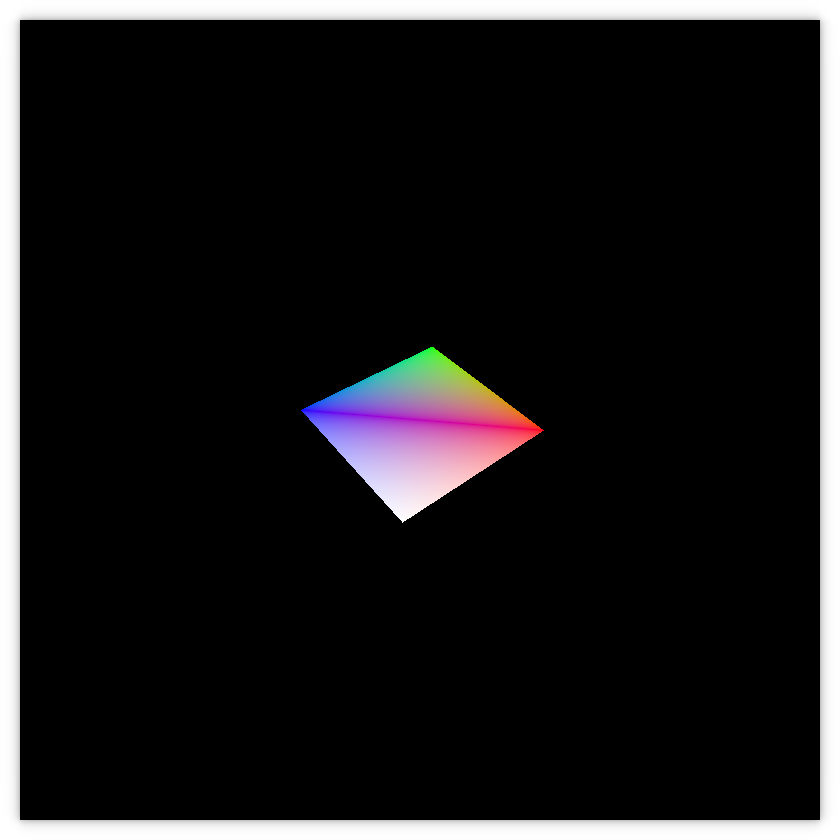
\includegraphics[width=0.25\textwidth]{images/3d.png}
    \caption{A flat plane after being transformed by the MVP}
\end{figure}

\subsubsection{Depth Testing}
Applying the MVP gave us a 3D scene, however objects were being rendered by draw order, meaning that objects that were farther away would be rendered on top of closer objects if they were lower down on the draw list, to fix this we implemented depth testing, depth testing is a specific render pass where the renderer draws a mask image that encodes an objects distance from the camera, the renderer can then use this image to only render the parts of faces that aren't being blocked by other objects.

In order to do this we needed to add another render pass that was set to measure depth, and saved in an image, this image was then plugged back into the graphics pipeline to ensure proper occlusion.

\begin{figure}[h]
    \centering
    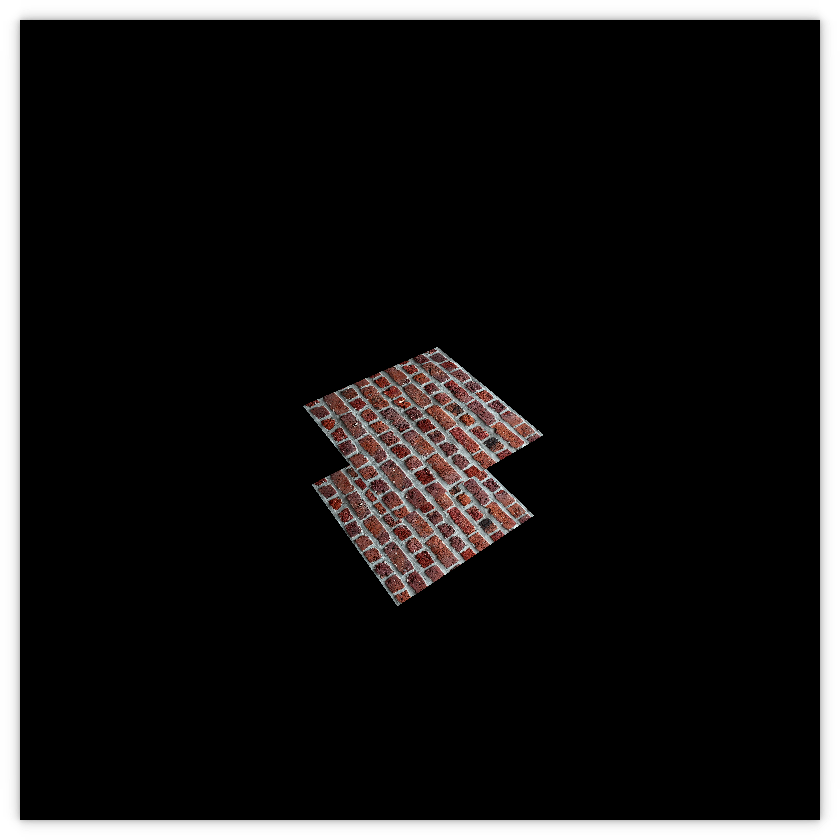
\includegraphics[width=0.25\textwidth]{images/depth.png}
    \caption{An example of proper depth testing}
\end{figure}

\subsubsection{Image sampling}
Up until this point, we were colouring objects per vertex, however, by providing an image texture and putting it through a sampler, we gain the ability to map an image onto faces.
Because the sampler is a shader input, it is implemented much in the same way as the uniform buffer object was, however, the principal difference in this case is that the sampler targets the fragment shader, as opposed to the buffer object which targets the vertex shader.

\begin{figure}[h]
    \centering
    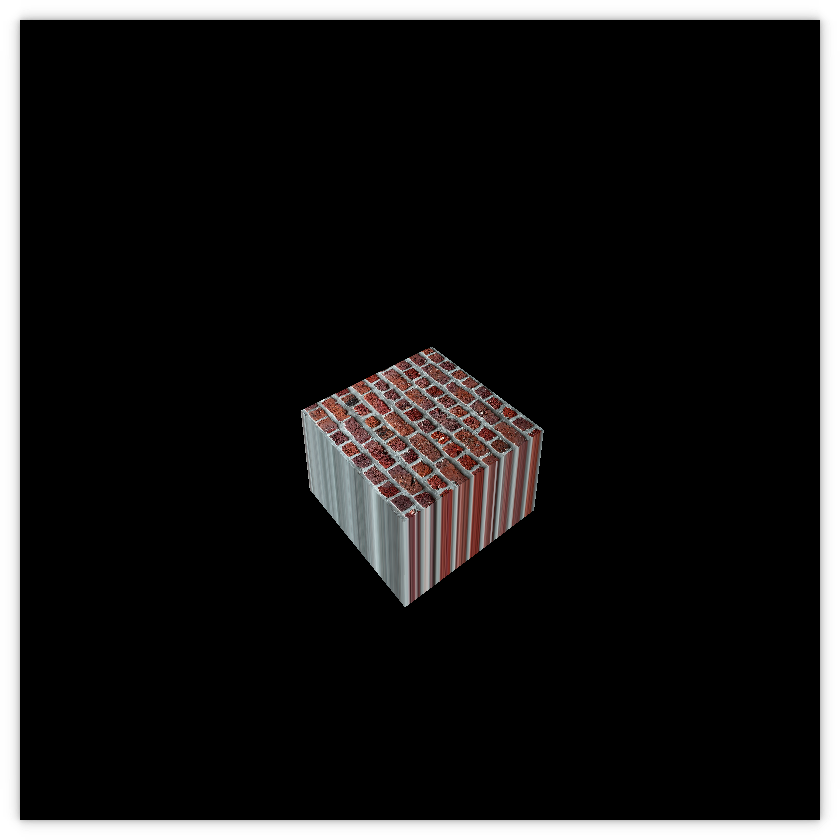
\includegraphics[width=0.25\textwidth]{images/cube.png}
    \caption{An image mapped onto a cube}
\end{figure}



\end{document}
